\chapter{差分隐私}\label{chap:differential-privacy}

2006年,Netflix 发起了一场全球竞赛,名为 Netflix Prize,旨在提升其电影推荐系统的精确度. 当时,Netflix 还主要是一家邮寄 DVD 的租赁服务公司,推荐系统对于帮助用户发现可能喜欢的电影至关重要. 为了激励全球数据科学家参与,Netflix 提供了100万美元的大奖,奖励给能将其推荐算法精度提高10\%的团队. 

Netflix 为比赛公开了一份庞大的数据集,包含超过一亿条匿名化的电影评分记录. 这些数据来自近五十万名用户,涉及约一万八千部电影. 为了保护隐私,Netflix 删除了所有直接的个人标识符,每个用户仅用一个随机的数字 ID 代替. 同时,性别、年龄、邮政编码等信息也被去除. 

然而,几周后,德克萨斯大学的博士生 Arvind Narayanan 和导师 Vitaly Shmatikov 证明,即使数据被匿名化,也能通过公开的互联网电影数据库(IMDb)进行去匿名化. 他们发现,攻击者只需掌握用户在几部电影上的评分和时间,就能在 Netflix 数据集中重新识别出这个用户. 这一发现揭示了严重的隐私风险. 

这个隐私问题导致了一起重要的诉讼案件. 一位未公开其性取向的同性恋母亲认为,Netflix 数据集的去匿名化可能会使她的性取向曝光,进而影响她的职业生涯和家庭生活. 她对 Netflix 提起了诉讼,要求 Netflix 根据《视频隐私保护法案》赔偿每位用户 2,500 美元,总计超过 5 亿美元. 最终,Netflix 与她达成了和解,并决定取消计划中的第二届 Netflix Prize 竞赛. 

直到2024年,Netflix也在也没有举办过第二届 Netflix Prize 竞赛,它的服务也已经转变到互联网上的在线视频为主. 然而,在当今世界,数据隐私的问题反而变得愈发严重. 我们每天看的在线视频、购物、社交网络等行为都会产生大量的数据,根据Statista在2020年的一项估计,2024年每人每天产生的数据量会达到63.5GB!然而,这些数据都被私人公司所掌握!

本章我们关心数据的另一个维度:社会属性. 尽管基于大数据和机器学习的技术的确改善了我们的生活,但是对数据的滥用也会带来严重的社会问题. 如何保护个体的隐私,同时又能够让机器学习得到足够的数据?\textbf{差分隐私}\index{差分隐私}就是解决这个问题的一个方法,本章将更详细地介绍差分隐私的概念和应用. 

\section{数据隐私问题}

本章开篇的Netflix Price案例展示了一个典型的数据隐私问题. 实际上,不仅资本需要数据,科研也极其需要数据. 以医学为例,我们需要大量真实的病人提供病情数据. 但这些数据可能都涉及到病人的隐私信息,例如一些\emph{敏感数据}. 因此,我们必须找到一种方法,既可以收集到这些数据,又保护病人的隐私信息.

保护病人的隐私信息的一种理解是不会让数据获得者将数据和人对应起来. 那么最直观的想法就是将每条\emph{数据匿名化}\index{数据匿名化}. 比如,每条数据只包含患者的生日、性别、邮政编号(代表位置\footnote{如果研究的是传染病,那么位置的意义也是很大的. })和病情.

这样做依然有问题:同一天生日、同一性别、相同邮政编号的人很少,而这些信息很容易被找到,比如,在家过生日的时候,在微博上分享了带定位的生日照. 通过一条数据的各种属性可以轻易定位到这个人,这样的匿名化是不安全的.

以上例子展现的是一种\emph{去匿名化}\index{去匿名化}的现象,也就是说匿名的数据实际上揭示了数据对应的那个个体. 这去匿名化的出现都是因为多维数据具有\emph{稀疏性},也就是说,尽管维数很高,但是同时满足多个条件的数据却很少. 

比如我们看\Cref{tab:tab01},这是医院甲的病人数据表. 56岁的病人只有赵丽娜,所以假如我们知道赵丽娜的年龄并了解到她去过这家医院,便立即得知她患有艾滋病.

\begin{table}[!ht]
\centering
\begin{tabular}{cccccc}
    \toprule
    \textbf{姓名} & \textbf{年龄} & \textbf{性别} & \textbf{邮政编码} & \textbf{是否吸烟} & \textbf{诊断} \\ \midrule
    李国强 & 64 & 男性 & 190146 & 是 & 心脏病 \\ 
    王秀英 & 61 & 女性 & 190118 & 否 & 关节炎 \\ 
    张建华 & 67 & 男性 & 190104 & 是 & 肺癌 \\ 
    陈玉兰 & 63 & 女性 & 190146 & 否 & 克罗恩病 \\ 
    刘志强 & 69 & 男性 & 190115 & 是 & 肺癌 \\ 
    赵丽娜 & \light{56} & 女性 & 190103 & 否 & 艾滋病 \\ 
    周志成 & 52 & 男性 & 190146 & 是 & 糖尿病 \\ 
    马文杰 & 59 & 男性 & 190130 & 是 & 过敏性鼻炎 \\ 
    李梅 & 55 & 女性 & 190146 & 否 & 溃疡性胃炎 \\ \bottomrule
    \end{tabular}

\caption{医院甲的病人数据表}
\label{tab:tab01}
\end{table}

类似\Cref{cha:J-L-Lemma},一种减少稀疏性的思想是\emph{降维},也就是我们用更粗糙的表示方法,但是让多维数据中同时满足多个条件的数据变得更多. 

具体到隐私的情景下,我们称之为\emph{$k$-匿名性}\index{$k$-匿名性}:任何一个人的信息都不能和其他至少$(k-1)$人区分开. 比如,可以不明确写出姓名、年龄和邮编,只给出模糊的范围,于是数据变成了下面的\Cref{tab:tab02}. 此时,有一个人的信息和赵丽娜完全相同,但是得了不同的病,这样赵丽娜的隐私就得到了保护.

\begin{table}[!ht]
\centering
\begin{tabular}{cccccc}
\toprule
    \textbf{姓名} & \textbf{年龄} & \textbf{性别} & \textbf{邮政编码} & \textbf{是否吸烟} & \textbf{诊断} \\ \midrule
    * & 60-70 & 男 & 1901** & 是 & 心脏病 \\ 
    * & 60-70 & 女 & 1901** & 否 & 关节炎 \\ 
    * & 60-70 & 男 & 1901** & 是 & 肺癌 \\ 
    * & 60-70 & 女 & 1901** & 否 & 克罗恩病 \\ 
    * & 60-70 & 男 & 1901** & 是 & 肺癌 \\ 
    \light* & \light{50-60} & \light{女} & \light{1901**} & \light{否} & 艾滋病 \\ 
    * & 50-60 & 男 & 1901** & 是 & 糖尿病 \\ 
    * & 50-60 & 男 & 1901** & 是 & 过敏性鼻炎 \\ 
    \light* & \light{50-60} & \light{女} & \light{1901**} & \light{否} & 溃疡性胃炎 \\ \bottomrule
\end{tabular}

\caption{医院甲的病人数据表,模糊了姓名、年龄和邮编}
\label{tab:tab02}
\end{table}

这种方法仍然存在问题,因为我们不能把关键信息(病症信息)也模糊化. 如果我们还拿到了另一家医院乙模糊之后的病人数据表(\Cref{tab:tab03}),那么依然有办法定位到赵丽娜. 这两张表上50-60岁的女性只有艾滋病是重合的,因此,如果我们知道赵丽娜的年龄并知道她同时去过两家医院,便立即得知她患有艾滋病.

\begin{table}[!ht]
\centering
\begin{tabular}{ccccc}
    \toprule
    \textbf{姓名} & \textbf{年龄} & \textbf{性别} & \textbf{邮政编码} & \textbf{诊断} \\\midrule
    * & \textcolor{Orchid}{50-60} & \textcolor{Orchid}{女} & 1901** & 艾滋病 \\ 
    * & \textcolor{Orchid}{50-60} & \textcolor{Orchid}{女} & 1901** & 系统性红斑狼疮 \\ 
    * & \textcolor{Orchid}{50-60} & \textcolor{Orchid}{女} & 1901** & 干燥综合征 \\ 
    * & 60-70 & 男 & 1901** & 胰腺癌 \\ 
    * & 60-70 & 男 & 1901** & 肝硬化 \\ 
    * & 60-70 & 男 & 1901** & 通风 \\ \bottomrule
    \end{tabular}
\caption{医院乙的病人数据表,模糊了姓名、年龄和邮编}
\label{tab:tab03}
\end{table}

除了使用匿名化的手段,还有一种方法可以保护隐私:不再提供单人的数据,而是直接公布将数据集的总体信息,比如平均值. 但这种方法也不一定能保证不泄露单人数据,请看下面的例子. 

在\Cref{sec:language-models} 中我们介绍过,要训练一个生成式语言模型(例如ChatGPT),需要大量的文本数据. 这些文本数据通常都是公司的机密,我们不得而知. 然而,我们可以用很简单的手段来推测这些数据. 

2023年12月27日,《纽约时报》因版权侵犯问题对OpenAI和微软提起诉讼. 该报指控这两家公司在训练其自动聊天机器人(即ChatGPT)时,未经许可使用了数百万篇《纽约时报》的文章. 这些聊天机器人如今被视为可信的信息来源,并与《纽约时报》等新闻机构展开了直接竞争. 

《纽约时报》在诉讼中提到几个实例,显示聊天机器人提供的内容几乎与《纽约时报》的文章完全一致,而这些文章在《纽约时报》的网站上需付费订阅才能阅读. 该报表示,OpenAI和微软特别强调在训练过程中使用了《纽约时报》的报道,因其认为这些材料具备可靠性和准确性. 

本案件如同罗生门,只要微软和OpenAI不主动承认,没有人可以证明他们确实使用了《纽约时报》的文章. 然而,这一案例足够说明一个道理:即使不提供模型本身,只提供模型的输出,也可能泄露出原始数据.

\begin{remark}
以上这些内容都说明\emph{匿名化}很难保护个人隐私. 那么,密码学\emph{加密}的手段是否能够保护隐私?比如说,为什么我们的所有数据不能需要账号密码才能被访问?其实,加密和隐私在出发点上完全不同. 

加密的目的是为了不让别人获取到真实数据. 而隐私不是简单地保护数据,它涉及更微妙的问题——我们希望利用这些数据,但是又不希望泄露某个个体的信息. 因此我们这里讨论的其实是隐私保护问题而不是加密问题,密码学的方案并不适用于这里.
\end{remark}

\section{差分隐私的定义与性质}

我们上面探讨了隐私保护的必要性以及它的微妙之处,现在我们要给出一种合理的方案解决隐私保护的问题,这个方案就是\emph{差分隐私}. 要给出一个数学模型,不仅要知道什么情况下算是隐私泄漏,也需要知道什么情况下不算,所以我们再来看一个反面的例子. 

李明是一位长期吸烟的男子,他参加了一项有关“吸烟与健康”的调查. 这项调查在不久后发布了一项结果,表明长期吸烟的人患上肺癌的几率更大. 伴随着这一结果的公布,保险公司在出售相同保险时会对长期吸烟者索要更高的价格. 李明当然也受到了这一政策的影响. 那我们是否可以认为这项研究泄露了李明的隐私(即更有可能患肺癌)呢?

直接告诉我们,这不应该算泄露了隐私. “长期吸烟的人患上肺癌的几率更大”这项结论并不依赖于李明是否参加了调查. 考虑这样的对照,$x$代表原来参加调查的人的集合,$x'$代表其他人不变,只是李明换成了另外一个人的集合. 如果是$x'$这些人参与了调查,结论是否会发生变化?\emph{大概率}不会!

李明的例子告诉我们,隐私应该有以下性质:
\begin{quotation}
    当数据集中包含李明的信息,相比数据集中不包含李明的信息,并不会\emph{显著}增加损害李明的利益的概率.
\end{quotation}
这一思想引出了\emph{差分隐私}\index{差分隐私}的概念,我们将在下面给出数学形式的定义.

考虑数据的空间$\mathcal X$,其中的每一个元素都包含了个体的所有可能数据例如姓名、性别、年龄、国籍等. 考虑$n$个人的数据,形成了有序的数据集
\[x = (x_1, \cdots, x_n) \in \mathcal X^n.\]  

我们希望对这些数据进行一定的加工,例如用这些数据来训练一个机器学习模型. 抽象来说,加工的过程可以被看成一个随机算法$A$:在固定输入数据集 $x \in \mathcal X^n$下,$A(x)$ 是输出空间 $\mathcal Y$ 上的一个随机变量. 

当我们改变(增加或删除)一个人的数据时,我们希望结果分布的变化可以控制在一定范围内. 为此,我们引入相邻数据集的概念:

\begin{definition}[$k$-相邻数据集]\index{$k$-相邻数据集}
    设 $x, x' \in \mathcal X^n$,如果 $x$ 和 $x'$ 最多有$k$条数据不同,即至多存在$k$个不同的$i_1,\dots,i_k \in [n]$ 使得 $x_{i_j}=x_{i_j}'$对$j\in[k]$成立,那么称 $x$ 和 $x'$ 是 \textbf{$k$-相邻的}. 
    
    特别地,如果$k=1$,我们称$x$和$x'$是\textbf{相邻的}.
\end{definition}

在李明的例子中,我们把李明换掉之前和之后的数据集是$1$-相邻的. 

接下来我们给出差分隐私的定义. 直观上,不论数据集中是否包含某个人的数据,算法的输出分布不会有太大的变化,因而我们有:

\begin{definition}[差分隐私,$\epsilon$-DP]\index{$\epsilon$-DP}\index{差分隐私}
考虑随机算法 $A : \mathcal X^n \to \mathcal Y$,如果对于任意一对$1$-相邻数据集$x, x'$,对任意(可测)值集 $E \subseteq \mathcal Y$,有
\[
\Pr(A(x)\in E) \leq \e^{\epsilon} \cdot \Pr(A(x')\in E),
\]
那么我们称$A$为\emph{数据集大小为 $n$ 的 $\epsilon$-DP算法}.
\end{definition}

这一定义看起来是不对称的,其实它是对称的,并且是用概率的比值衡量分布的差异. 

\begin{proposition}
    设$A:\mathcal X^n\to\mathcal Y$是一个$\epsilon$-DP算法,那么对于任意的$1$-相邻数据集$x, x'$和任意(可测)值集 $E \subseteq \mathcal Y$,有
    \[
    e^{-\epsilon}\leq \frac{\Pr(A(x)\in E)}{\Pr(A(x')\in E)}\leq \e^{\epsilon}.
    \]
\end{proposition}
\begin{proof}
    不等式右边就是定义,左边只需要把定义中$x$和$x'$的地位互换即可.
\end{proof}

从这一性质出发,如果$\epsilon$越接近$0$,那么$A$的输出分布在相邻数据集上的变化就越小,也就是说隐私保护效果越好.

\begin{remark}
    为什么选择用比值来衡量分布的差异,而不是直接用差值?注意,如果我们要讨论对数据的多重加工,那么加工之间的\emph{独立性}就是一个很重要的性质. 独立性的定义就使用了乘法(也就是比值),而不是加法. 因此,我们将在后面看到,这样定义的差分隐私具有极其干净的数学性质. 
\end{remark}

以上定义需要对所有的(可测)值集$E$都成立,这给验证带来了极大的困难,如果随机算法的输出分布是更加常规的,我们可以简化验证的过程. 

对于离散型的输出,我们有如下等价定义:
\begin{proposition}\label{prop:discrete-dp}
    如果 $A(x)$对于任意 $x \in \mathcal X^n$ 都是离散型随机变量,那么随机算法$A$是数据集大小为 $n$ 的 $\epsilon$-DP算法当且仅当对于任意一对$1$-相邻数据集$x, x'$和所有的 $y \in \mathcal Y$,有
    \[
    \Pr(A(x) = y) \leq \e^{\epsilon} \cdot \Pr(A(x') = y).
    \]
\end{proposition}
\begin{proof}
$\implies$:取$E = \{y\}$即可证明.

$\impliedby$:假设$E=\{y_1,\dots,y_k,\dots\}\subseteq\mathcal Y$. 对每一个$y_i$,都有
    \[
    \Pr(A(x) = y_i) \leq \e^{\epsilon} \cdot \Pr(A(x') = y_i).
    \]
因为$A(\cdot)=y_i$对于不同的$i$是互斥事件,所以概率可以直接相加,于是:
    \begin{align*}
    \Pr(A(x) \in E) &= \sum_i \Pr(A(x) = y_i) \\
    &\leq \e^{\epsilon} \cdot \sum_i\Pr(A(x') = y_i) \\
    &= \e^{\epsilon} \cdot \Pr(A(x') \in E).
    \end{align*}
\end{proof}

对连续型的输出,我们有如下等价定义:
\begin{proposition}\label{prop:continuous-dp}
如果 $A(x)$对于任意 $x \in \mathcal X^n$ 都是连续型随机变量,那么它存在概率密度函数,记为$h_{x}$. 此时,随机算法$A$是数据集大小为 $n$ 的 $\epsilon$-DP算法当且仅当对于任意一对$1$-相邻数据集$x, x'$和几乎所有的 $y \in \mathcal Y$,有
    \[
    h_{x}(y) \leq \e^{\epsilon} \cdot h_{x'}(y).
    \]
\end{proposition}
\begin{proof}
$\implies$:这一部分的严格表述需要测度论的基础,所以这一证明从直观上理解即可,不需要考虑严格的定义. 如果需要看更严格的定义,请参阅\Cref{chap:prob}.

定义集合
\[E=\{y:h_x(y)>\e^\epsilon\cdot h_{x'}(y)\}.\]
我们证明$\lambda(E)=0$,其中$\lambda$是Lebesgue测度;也就是说,几乎所有的$y$都满足
\[h_x(y)\leq\e^\epsilon\cdot h_{x'}(y).\]
为此,我们定义集合
\[E_n=\left\{y:h_x(y)>\e^\epsilon\cdot h_{x'}(y)+\frac{1}{n}\right\}, n=1,2,\dots.\]
因为
\[E=\bigcup_{n=1}^\infty E_n,\]
所以我们只需要证明$\lambda(E_n)=0$,然后利用测度的次可加性即可证明$\lambda(E)=0$.

假设$\lambda(E_n)>0$,那么,在$E_n$上对密度函数积分,有
\[\int_{E_n}(h_x(y)-\e^\epsilon\cdot h_{x'}(y))\d y\geq \int_{E_n}\frac{1}{n}\d y=\frac{\lambda(E_n)}{n}>0.\]
根据概率密度的定义,
\[\Pr(A(x)\in E_n)=\int_{E_n}h_x(y)\d y,\quad\Pr(A(x')\in E_n)=\int_{E_n}h_{x'}(y)\d y.\]
所以
\[\Pr(A(x)\in E_n)>\e^\epsilon\cdot\Pr(A(x')\in E_n).\]
这与$A$是$\epsilon$-DP算法矛盾,所以$\lambda(E_n)=0$,这就完成了证明.

$\impliedby$:依然根据概率密度函数的定义,考虑$x,x'\in\mathcal X^n$,对任意可测$E\subseteq\mathcal Y$,有
\begin{align*}
\Pr(A(x)\in E) &= \int_E h_x(y)\d y \\
&\leq \e^\epsilon\cdot\int_E h_{x'}(y)\d y \\
&= \e^\epsilon\cdot\Pr(A(x')\in E).
\end{align*}
\end{proof}

接下来我们给出差分隐私的基本性质. 首先,如果我们对一组数据$x$依次独立使用两个差分隐私算法$A_1$和$A_2$进行处理(允许$A_2$使用$A_1$输出的结果),得到两组数据,那么总体上看,这整个过程还是一个差分隐私算法. 

\begin{proposition}[复合性,两个算法的情形]\label{prop:composition}\index{差分隐私!复合性}
    $A_1$ 和 $A_2$ 是相互独立的随机算法,其中 
    \begin{align*}
        A_1&: \mathcal X^n \to \mathcal Y_1,\\
        A_2&: \mathcal Y_1 \times \mathcal X^n \to \mathcal Y_2.
    \end{align*}
    假设$A_1$是 $\epsilon_1$-DP算法,$A_2$ 是 $\epsilon_2$-DP算法.
    
    令 $A :\mathcal X^n \to \mathcal Y_1 \times \mathcal Y_2$ 是随机算法,输出为 $A(x) = (y_1, y_2)$,其中 $y_1 = A_1(x)$, $y_2 = A_2(y_1, x)$,那么 A 是$(\epsilon_1 + \epsilon_2)$-DP算法.
\end{proposition}

\begin{proof}
为了简化记号,这里我们只证明离散的情况,一般情况的证明类似. 令 $x,x'$ 是 $\mathcal X^n$ 中的两个$1$-相邻数据集,$A$输出为 $y = (y_1, y_2) \in \mathcal Y_1 \times \mathcal Y_2$,那么根据定义和独立性,
    \[
    \Pr(A(x) = (y_1, y_2)) = \Pr(A_1(x) = y_1) \cdot \Pr(A_2(y_1, x) = y_2).
    \]
由于 $A_1$ 是 $\epsilon_1$-DP算法,$A_2$是 $\epsilon_2$-DP算法,得到
    \[
    \begin{aligned}
        \Pr(A(x) = (y_1, y_2)) &= \Pr(A_1(x) = y_1) \cdot \Pr(A_2(y_1, x) = y_2)\\
        &\leq \e^{\epsilon_1} \Pr(A_1(x') = y_1) \cdot \e^{\epsilon_2} \Pr(A_2(y_1, x') = y_2) \\
        &= \e^{\epsilon_1 + \epsilon_2} \cdot \Pr(A(x') = (y_1, y_2)).
    \end{aligned}
    \]
\end{proof}

现在,我们已经看到为什么差分隐私的定义是用比值来衡量的:比值陈述的差分隐私,这一命题的结论和证明都非常干净. 利用数学归纳法,很容易推广到多个随机算法的复合性:

\begin{proposition}[复合性,多个算法的情形]\label{prop:composition-multi}\index{差分隐私!复合性}
    设 $A_1, A_2, \cdots , A_k$ 为一列相互独立的随机算法, 
    \begin{align*}
        A_1&: \mathcal X^n \to \mathcal Y_1,\\
        A_i&: \mathcal Y_1 \times \cdots \times \mathcal Y_{i-1} \times \mathcal X^n \to \mathcal Y_i,\quad i = 2, 3, \cdots, k.
    \end{align*}
    也就是 $A_i$ 将 $A_1, \cdots, A_{i-1}$ 的输出和 $\mathcal X^n$ 中的一个数据集作为输入元素. 对$i=1,\dots,k$, $A_i$是 $\epsilon_i$-DP算法. 
        
    依次运行算法 $A_i$ 得到算法$A : \mathcal X^n \to \mathcal Y_1 \times \cdots \times \mathcal Y_k$,那么$A$是$\epsilon$-DP,其中$\epsilon = \sum_{i=1}^n \epsilon_i$.
\end{proposition}
\begin{proof}
    对$n$用数学归纳法. 
    \begin{itemize}
        \item 当$n=1$时,结论显然成立.
        \item 假设结论对$n$成立,我们要证明对$n+1$结论成立.
        
        考虑前$n$个算法的复合算法
        \[A'(x) = (A_1(x), A_2(A_1(x), x), \cdots, A_n(A_{n-1}(\cdots A_1(x), \cdots), x)).\]
        由归纳假设,$A'$是$\sum_{i=1}^n\epsilon_i$-DP算法. 
        
        由于$A_{n+1}$是$\epsilon_{n+1}$-DP算法,$A'$与$A_{n+1}$的复合算法是$A$,所以利用\Cref{prop:composition},$A$是$\sum_{i=1}^{n+1}\epsilon_i$-DP算法.
    \end{itemize}
\end{proof}

接下来,我们说明差分隐私最关键的性质:一旦被差分隐私算法处理过,无论后续如何处理,都不会影响隐私保护的效果.

\begin{proposition}[后处理]\label{prop:post-processing}\index{差分隐私!后处理}
    令 $A : \mathcal X^n \to \mathcal Y$, $B : \mathcal Y \to \mathcal Z$ 为相互独立的随机算法,其中 $\mathcal X$, $\mathcal Y$, $\mathcal Z$ 是任意集合. 如果 $A$ 是 $\epsilon$-DP算法,那么复合算法$ B(A(\cdot))$ 也是 $\epsilon$-DP算法.
\end{proposition}
\begin{proof}
我们仍然只考虑离散情形,采用定义的方法证明
    \[
    \begin{aligned}
        \Pr(B(A(x)) = b) &= \sum_{y \in \mathcal Y} \Pr(A(x) = y) \Pr(B(y) = b) \\
        &\leq \e^{\epsilon} \sum_{y\in \mathcal Y}\Pr(A(x') = y)\Pr(B(y) = b)\\
        &= \e^{\epsilon}\Pr(B(A(x')) = b).
    \end{aligned}
    \]
\end{proof}

最后,我们讨论如果有多个人的数据都发生变化的时候,隐私保护的性质会发生什么变化. 

\begin{proposition}[群体隐私]\label{prop:group-privacy}\index{差分隐私!群体隐私}
    令 $x, x' \in \mathcal X^n$ 是$k$-相邻数据集,$1 \leq k \leq n$. 如果 $A$ 是 $\epsilon$-DP算法,那么对所有的值集$E$,我们有
    \[
    \Pr(A(x) \in E) \leq \e^{k\epsilon}\Pr(A(x') \in E).
    \]
\end{proposition}
\begin{proof}
    考虑数据集 $x_0, x_1, \cdots , x_k$,其中 $x_0 = x$, $x_k = x'$,且 $x_i$ 和 $x_{i+1}$ 是$1$-相邻数据集,$i = 0, \cdots, k-1$. 那么
    \[
    \begin{aligned}
    \Pr(A(x) \in E) &\leq \e^{\epsilon}\Pr(A(x_1) \in E) \leq \e^{2\epsilon}\Pr(A(x_2) \in E)\\
    &\leq \cdots \leq \e^{k\epsilon}\Pr(A(x') \in E).
    \end{aligned}
    \]
\end{proof}

换言之,$k$-相邻数据集上$\epsilon$-DP算法的表现仿佛一个$k\epsilon$-DP算法. 

这一性质还可以推出$\epsilon$的含义. 我们知道,数据集$x, x' \in \mathcal X^n$最多在$n$个位置不同. 所以对于一个$\epsilon$-DP算法$A$,一定有
        \[
        \Pr(A(x) \in E) \leq \e^{n\epsilon}\Pr(A(x') \in E).
        \]
如果$\epsilon$太小,这一算法对任何输入都有相似的输出. 换句话说,算法压根没有输出任何有意义的内容. 于是,我们定量说明了,$\epsilon$还代表信息的泄露量. 因此,一个实用的DP算法不能让$\epsilon$太小,否则输出没有意义;也不能让$\epsilon$太大,否则隐私保护效果不好.

\section{差分隐私的应用}
在这一部分,我们将会具体讨论三个差分隐私的算法或机制. 

\subsection{随机反应算法}
我们从一个具体场景开始. 假设有一名老师想要调查班上的同学有多少人曾经在考试中作弊. 设班上一共有$n$名同学,每个人的真实答案是一个数字$x_i \in \{0,1\}$,$0$表示没有作弊,$1$表示作弊. 

没有人愿意主动承认自己作弊,所以,对于每个$i$,独立地按照以下规则根据$x_i$得到对应的$y_i$:
\[\begin{aligned}
    y_i =
    \begin{cases}
        x_i, & \text{ 以$2/3$的概率 }, \\
        1 - x_i,& \text{ 以$1/3$的概率}.
    \end{cases}
\end{aligned}\]
然后,老师让每个同学回答$y_i$,并公布$\sum_{i=1}^n y_i$. 

这的确可以保护隐私:当$y_i = 1$时,学生$i$可以声称这是由于算法的随机机制造成的,而并非自己真的作弊过,因而他愿意诚实回答. 

我们称这一算法为\emph{随机反应}(RR)算法\index{随机反应算法}\index{RR算法},它是S. L. Warner在1965年提出的(远远早于差分隐私概念的提出!),被广泛用于调查敏感问题.

以下结论说明了RR算法的确是差分隐私算法.

\begin{theorem}
    RR 算法是 $\log 2$-DP算法.
\end{theorem}
\begin{proof}
记$Y_i$是$y_i$对应的随机变量. 我们知道$y_i$之间相互独立,所以
    \[
    \Pr(A(x) = y) = \prod_{i=1}^n \Pr(Y_i = y_i  | x_i).
    \]
对于$y_i$,我们有
    \[
    \frac{\Pr(Y_i = y_i  | x_i = y_i)}{\Pr(Y_i = y_i  | x_i = 1 - y_i)} = \frac{2/3}{1/3} = 2.
    \]
类似地,我们有
    \[
    \frac{\Pr(Y_i = y_i  | x_i = 1 - y_i)}{\Pr(Y_i = y_i  | x_i = y_i)} = \frac{1/3}{2/3} = 1/2.
    \]

所以,对于一对$1$-相邻数据集$x, x'$和任意的$y \in \mathcal Y$,假设$x_j \neq x'_j$,不论$y_j$,$x_j$和$x'_j$的取值是什么,我们都有
    \begin{align*}
    & \frac{\Pr(A(x) = y)}{\Pr(A(x') = y)} \\
    =& \frac{\prod_{i=1}^n \Pr(Y_i = y_i  | x_i)}{\prod_{i=1}^n \Pr(Y_i = y_i  | x'_i)} \\
    =& \frac{\Pr(Y_j = y_j  | x_j)}{\Pr(Y_j = y_j  | x'_j)}\leq 2.
    \end{align*}
由\Cref{prop:discrete-dp},RR算法是$\log 2$-DP算法.
\end{proof}

另一方面,我们真正关心的是$\sum_{i=1}^n x_i$,也就是有多少人作弊. 我们希望RR算法的输出能够很好地估计出这一值,也就是RR算法得到的$\sum_{i=1}^n Y_i$是否能很好的估计出$\sum_{i=1}^n x_i$. 

为此,假设每个人独立地有$p$的概率作弊,那么从期望上说,作弊的人大概有$np$个,但我们不知道$p$. 假设每个人的真正回答是随机变量$Y_i$,我们来计算$\E[\sum_{i=1}^n Y_i]$.
\begin{align*}
    \E[Y_i]=\Pr(Y_i = 1) &= p \cdot \frac23 + (1 - p) \cdot \frac13 \\
    \implies p &= 3\E[Y_i] - 1.
\end{align*}
对$i$累和,我们有
\[
    np=3\E\left[\sum_{i=1}^n Y_i\right] - n.
\]
所以,RR算法的输出$\sum_{i=1}^n y_i$在期望上很好地估计了$\sum_{i=1}^n x_i$.

\subsection{全局灵敏度与Laplace机制}

RR算法是如何实现差分隐私的呢?最重要的一步是,它把真实数据加了噪声,但是这一噪声并不会过分地影响结果. 更一般地,我们似乎总是可以通过向输出添加噪声来实现差分隐私. 那么就引出了另一个问题,需要添加多大的噪声?

一个极端是,如果我们添加的噪声太大,那么输出就完全变成随机的了;另一个极端是,我们完全不加噪声,这样就没有隐私保护的效果. 我们希望能够找到一个合适的噪声水平,使得既能保护隐私,又能保持输出的有用性. 多大的噪声合适,这和算法本身的性质有关,比如,当输入只改变一点时,算法的输出会改变多大?我们定义全局灵敏度来衡量这一性质.

\begin{definition}[全局灵敏度]\index{全局灵敏度}
给定算法$f: \mathcal X^n \to \R$,定义$f$的\textbf{全局灵敏度}为
    \[
    \mathsf{GS}_f = \sup_{x, x' \text{ 在 }\mathcal X^n\text{ $1$-相邻}} |f(x) - f(x')|. 
    \]
\end{definition}
定义中的$1$-相邻,可能会随着情景不同而改变. 全局灵敏度的定义是很直观的,就是改变一条数据会对算法输出带来的最大可能变化. 

我们来计算一个简单的例子.
\begin{example}
设$f(x)= \frac1n \sum_{i=1}^n \phi(x_i)$,$\phi : \mathcal X\to [0,1]$是满射. 那么,
\begin{align*}
    \mathsf{GS}_f&=\sup_{x, x' \text{ 在 }\mathcal X^n\text{ $1$-相邻}} |f(x) - f(x')|\\
    &= \sup_{x, x' \text{ 在 }\mathcal X^n\text{ $1$-相邻}} \frac1n \left|\sum_{i=1}^n \phi(x_i) - \sum_{i=1}^n \phi(x'_i)\right|\\
    &= \sup_{x, x' \text{ 在 }\mathcal X^n\text{ 只在 } j\text{ 不同}} \frac1n \left|\phi(x_j) - \phi(x'_j)\right| = \frac1n.
\end{align*}
\end{example}

接下来,我们试图给出一个一般的方法来构造差分隐私算法. 给定一个数据集$x \in \mathcal X^n$ 和参数$\epsilon$. 对于一个算法$f:\mathcal X^n \to \R$,我们想要给$f$的输出加一个噪声$Z$,使它具有差分隐私的性质. 新得到的算法$A$是一个随机算法,给定数据集$x$,它输出
\[
    A(x)=f(x)+Z.
\]

设$x$,$x'$是两个$1$-相邻数据集,记$\mu = f(x)$,$\mu' = f(x')$. 如果$Z$是连续型随机变量,我们希望密度函数$h_{x}$和$h_{x'}$满足
\[
    \frac{h_{x}(y)}{h_{x'}(y)} \leq \e^{\epsilon}.
\]

如何选择这样的$Z$呢?注意,$A(x)$和$A(x')$的只差一个常数$\mu - \mu'$,所以密度函数$h_{x}$和$h_{x'}$应该是关于$y$的平移,也就是
\[
    h_{x}(y) = h_{x'}(y - (\mu - \mu')).
\]
因为我们想要构造$\e^\epsilon$,所以不妨设想$Z$的密度函数具有指数$\e^{-x}$的形式\footnote{在此时,我们先不管它是不是密度函数,而是看如何才能够造出来差分隐私算法.},我们就会有
\[
    \frac{h_{x}(y)}{h_{x'}(y)} = \frac{h_{x'}(y - (\mu - \mu'))}{h_{x'}(y)} = \e^{(\mu - \mu')}.
\]
如果我们想要$\epsilon$-DP,那么我们就需要让$Z$的扰动不要太大. 如果用$\alpha Z$来替代$Z$,那么
\[
    \frac{h_{x}(y)}{h_{x'}(y)} = \e^{\alpha(\mu - \mu')}.
\]
注意到,$|\mu - \mu'| \leq \mathsf{GS}_f$,所以我们需要$\alpha \leq \epsilon/\mathsf{GS}_f$.

以上推导过程虽然不是严格的,但是它给出了我们构造差分隐私算法的一个思路,这一思路的最终结果为\emph{Laplace机制}\index{Laplace机制}. 首先引入Laplace分布的概念.

\begin{definition}[Laplace分布]\index{Laplace分布}
    给定参数$\mu\in\R$和$\lambda>0$,定义概率密度函数
        \[h(x  | \mu, \lambda) = \frac1{2\lambda}\exp\left(- \frac{|x - \mu|}{\lambda}\right).\]
我们称具有这一密度的分布为\emph{Laplace分布},记为$\mathsf{Lap}(\mu,\lambda)$.
\end{definition}

Laplace分布是服从双边指数分布的随机变量进行线性变换后服从的分布. 具体来说,设$X\sim\mathsf{DExp}(1)$,那么$\lambda X+\mu\sim\mathsf{Lap}(\mu,\lambda)$. 在\Cref{fig:Laplace-distribution} 中,我们展示了不同参数的Laplace分布密度函数图像. 更多关于Laplace分布的性质,我们留做习题. \lhysays{习题}

\begin{figure}[ht]
    \centering
    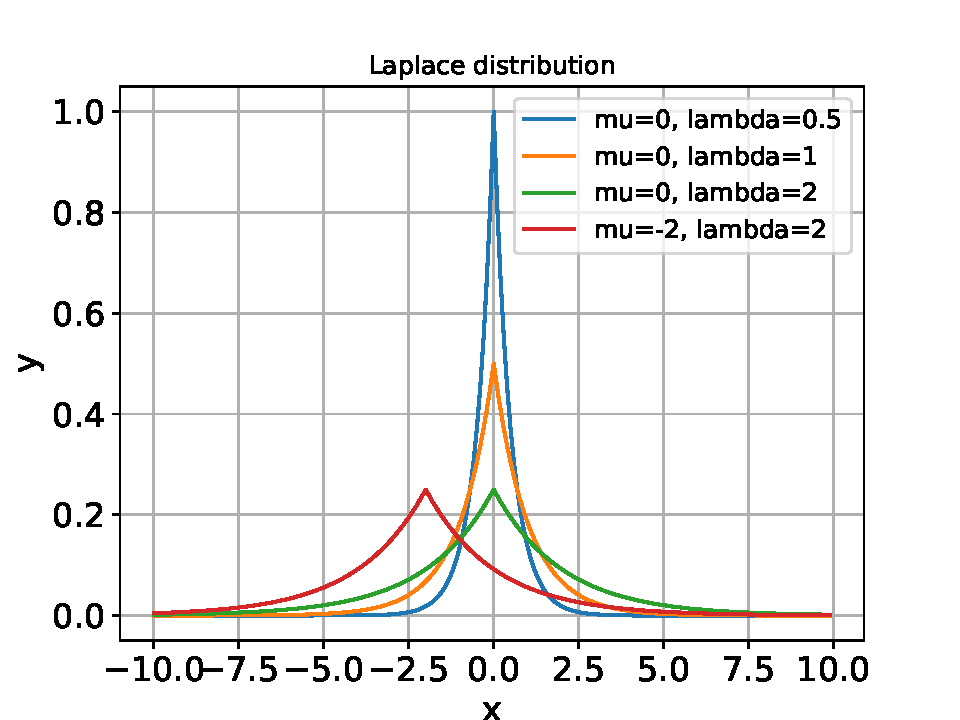
\includegraphics[scale=0.6]{Figures/differential-privacy/LaplaceDist.pdf}
    
    \lhysays{重画}
    \caption{Laplace分布的密度函数图像}
    \label{fig:Laplace-distribution}
\end{figure}

下面我们来陈述Laplace机制.

\begin{itemize}
    \item 给定算法$f:\mathcal X^n \to \R$,参数$\epsilon>0$.
    \item 计算全局灵敏度$\mathsf{GS}_f$.
    \item 构造随机算法$A_{\mathsf{Lap}}(x;\epsilon) = f(x) + Z$,其中$Z\sim \mathsf{Lap}(0, \mathsf{GS}_f/\epsilon)$.
\end{itemize}
如此,我们就得到了一个随机算法$A_{\mathsf{Lap}}$. 

\begin{theorem}\label{thm:laplace-mechanism}
    对于任意的$\epsilon > 0$,$A_{\mathsf{Lap}}$是$\epsilon$-DP算法.
\end{theorem}
\begin{proof}
设$x$,$x'$是两个$1$-相邻数据集,记$\mu = f(x)$,$\mu' = f(x')$. 由Laplace分布的性质可知,$A_{\mathsf{Lap}}(\epsilon, x) \sim \mathsf{Lap}(\mu, GS_f/\epsilon)$,$A_{\mathsf{Lap}}(\epsilon, x') \sim \mathsf{Lap}(\mu', GS_f/\epsilon)$.

因此,对于任意的$y \in \mathcal Y$,有
    \[
    \begin{aligned}
        \frac{h_{x}(y)}{h_{x'}(y)} &=\exp \left(-\epsilon \frac{|\mu - y| - |\mu' - y|}{GS_f} \right) \\
        &\leq \exp \left(\epsilon \frac{|\mu - \mu'|}{GS_f} \right)\leq \exp(\epsilon).
    \end{aligned}
    \]
根据\Cref{prop:continuous-dp},命题得证. 
\end{proof}

\subsection{DP版本Llyod算法}
作为一个Laplace机制的具体实例,我们将$k$-均值聚类问题的经典算法Llyod算法改造成一个差分隐私算法.

\emph{$k$-均值}\index{$k$-均值}聚类问题指的是给定一个数据集$x$,找到$k$个点(中心)$\{c_i\} \subseteq \R^d$,使得$\sum_{i \in [n]} \min_{j\in[k]} \norm{x_i - c_j}^2$最小. 通俗来说,就是找到$k$个中心,使得数据集中每个点到最近的中心的距离之和最小. 

在我们开始讨论算法和改造之前,我们先要理解为什么$k$-均值问题需要差分隐私. 我们可以把每一个点看作一个人的数据,而中心看作是一个数据集的平均特征. 我们只希望算法可以知道数据的平均特征,而不希望泄露某个个人的数据. 因此,我们希望$k$-均值算法是差分隐私的.

$k$-均值问题最常见的解决方法是使用迭代的启发式的\emph{Lloyd算法}\index{Lloyd算法},其表述为下:
\begin{itemize}
    \item 输入:数据集$x \in \mathcal X^n$,这里$\mathcal X = \{x \in \R^d : \norm{x}_1 \leq 1 \}$,参数$k$,最大迭代次数$T$.
    \item 随机初始化$c_1^{(0)}$, $c_2^{(0)}$, $\cdots$, $c_k^{(0)} \in \mathcal X$.
    \item for $t=1$ to $T$
    \begin{itemize}
        \item for $j=1$ to $k$
        \begin{itemize}
            \item 计算$S_j = \{i : c_{j}^{(t-1)} \text{ 是\ } x_i \text{ 最近的中心}\}$.
            \item 计算$n_j = |S_j|$.
            \item 计算$a_j = \sum_{i\in S_j} x_i$.
            \item 更新$c_j^{(t)} = a_j/n_j$.
        \end{itemize}
    \end{itemize}
    \item 输出:$c_1^{(T)}$, $c_2^{(T)}$, $\cdots$, $c_k^{(T)}$.
\end{itemize}

这一算法的思路大致是:首先随机初始化$k$个中心$c_i$,然后,对每一个$c_i$,找到离它最近的那些点,以这些点的平均值(也就是质心)作为新的$c_i$,重复这一过程直到收敛.

注意,如果初始化的中心就是各个质心,那么Llyod算法就已经找到最优解了. 事实上,可以证明,Llyod算法最终会收敛到最优解. 

尽管Llyod算法可以达到很好的效果,但它并不能保证DP性质. 我们希望对这一算法进行小规模的修改,让它具有$\epsilon$-DP的性质. 我们给出如下的DP版本Llyod算法.

\begin{itemize}
    \item 输入:数据集$x \in \mathcal X^n$,这里$\mathcal X = \{x \in \R^d : \norm{x}_1 \leq 1 \}$,参数$k$,最大迭代次数$T$,\textcolor{Orchid}{参数$\epsilon$}.
    \item \textcolor{Orchid}{$\epsilon' = \frac{\epsilon}{2 T}$},随机初始化$c_1^{(0)}$, $c_2^{(0)}$, $\cdots$, $c_k^{(0)} \in \mathcal X$.
    \item for $t=1$ to $T$
    \begin{itemize}
        \item for $j=1$ to $k$
        \begin{itemize}
            \item 计算$S_j = \{i : c_{j}^{(t-1)} \text{ 是 } x_i \text{ 最近的中心}\}$.
            \item $n_j = |S_j|$.
            \item $a_j = \sum_{i\in S_j} x_i$.
            \item \textcolor{Orchid}{计算 $\hat{n_j} = n_j + Y$,$Y \sim \mathsf{Lap}(0, 2/\epsilon')$.}
            \item \textcolor{Orchid}{计算 $\hat{a_j} = a_j + (Z_1, \cdots, Z_d)$,$Z_i \text{ i.i.d.}\sim \mathsf{Lap}(0, 2/\epsilon')$.}
            \item 更新
            $\begin{aligned}
            c_j^{(t)} =
            \begin{cases}
                \textcolor{Orchid}{\hat{a_j}/\hat{n_j}}, & \hat{n_j} \geq 1, \\
                \mathcal X\text{ 上的一个随机均匀采样}, & \hat{n_j} < 1.
            \end{cases}
            \end{aligned}$
        \end{itemize}
    \end{itemize}
    \item 输出:$c_1^{(T)}$, $c_2^{(T)}$, $\cdots$, $c_k^{(T)}$.
\end{itemize}

简单来说,我们对原来Llyod算法中产生的中间值都是用Laplace机制来加噪声,最终得到的中心也是加了噪声的. 以下定理表明上面的算法确实是一个$\epsilon$-DP算法. 
\begin{theorem}
    DP 版本的 Lloyd算法是$\epsilon$-DP算法.
\end{theorem}

\begin{proof}[证明概要]
我们只在这里陈述证明的大致想法,将细节留到习题\lhysays{习题}.

首先,作为一个迭代算法,我们可以把每轮迭代看成一次算法$A_t$的执行,而整个算法是这些算法的复合,整个算法一共有$T$次复合. 由\Cref{prop:composition-multi},我们只需要证明每一轮迭代是$(\epsilon/T)$-DP算法,那么整个算法就是$\epsilon$-DP算法.

进一步,考虑证明每一个$A_t$是$(\epsilon/T)$-DP算法. 每一个$A_t$内部都是$k$个独立的Laplace机制,实际上是一个输入为$n_j,a_j$,输出为$\hat{n}_j$,$\hat{a}_j$的算法. 所以,只需要证明:每一个独立Laplace机制确实是$(\epsilon/T)$-DP,然后再证明这些独立的Laplace机制总和的效果依然是$(\epsilon/T)$-DP,我们就可以证明整个命题.
\end{proof}

\section{习题}

\section{章末注记}
